% This document describes how to use iiscthesis style
%%%%%%%%%%%%%%%%%%%%%%%%%%%%%%%%%%%%%%%%%%%%%%%%%%%%%%%%%%%%%%%%%%%%%%%%%%%
\documentclass[12pt]{iiscthes} %Changed documentstyle to documentclass to upgrade the document to LaTex2e.

\usepackage{thesis_preamble}
%\pagestyle{bfheadings}


% https://ctan.org/pkg/mylatexformat - Check this for faster rendering

% Put your macros here
%\newfont{\punkbx}{punkbx20}

% To render faster use \includeonly. https://en.wikibooks.org/wiki/TeX/includeonly
%\includeonly{Chapters/1.Introduction/Introduction}

\begin{document}

%%%%%%%%%%%%%%%%%%%%%%%%%%%%%%%%%%%%%%%%%%%%%%%%%%%%%%%%%%%%%%%%%%%%%%%%%%%
% The frontmatter environment for everything that comes with roman numbering
\begin{frontmatter}
%                         THE TITLEPAGE                              %
%%%%%%%%%%%%%%%%%%%%%%%%%%%%%%%%%%%%%%%%%%%%%%%%%%%%%%%%%%%%%%%%%%%%%%

\title{Primary Alpha, Transformed Beta and Low Cycle Fatigue of Titanium Alloys (Ti6242 and Ti6246)}
\author{Sharan Chandran}
% For all the parameters below, take default values
\submitdate{August}
\dept{Materials Engineering}
\enggfaculty
%\degreein{Computer Science and Engineering}
%\mscengg
%\me
\iisclogotrue % Default is false
% \figurespagefalse %default is true
\tablespagetrue %default is false
\maketitle
%%%%%%%%%%%%%%%%%%%%%%%%%%%%%%%%%%%%%%%%%%%%%%%%%%%%%%%%%%%%%%%%%%%%%%
%                              COPYRIGHT                             %
% Copyright is automatically included by the style file              %
%%%%%%%%%%%%%%%%%%%%%%%%%%%%%%%%%%%%%%%%%%%%%%%%%%%%%%%%%%%%%%%%%%%%%%


%%%%%%%%%%%%%%%%%%%%%%%%%%%%%%%%%%%%%%%%%%%%%%%%%%%%%%%%%%%%%%%%%%%%%%
%                              DEDICATION                            %
%%%%%%%%%%%%%%%%%%%%%%%%%%%%%%%%%%%%%%%%%%%%%%%%%%%%%%%%%%%%%%%%%%%%%%
\begin{dedication}
% You can design this page as you like
\begin{center}
TO \\[2em]
\large\it Donald Knuth\\
and\\
\large\it His Ingenuity 
\end{center}
\end{dedication}
%%%%%%%%%%%%%%%%%%%%%%%%%%%%%%%%%%%%%%%%%%%%%%%%%%%%%%%%%%%%%%%%%%%%%%
%                         ACKNOWLEDGEMENTS                           %
%%%%%%%%%%%%%%%%%%%%%%%%%%%%%%%%%%%%%%%%%%%%%%%%%%%%%%%%%%%%%%%%%%%%%%
\acknowledgements

Many thanks to all the persons who made this style file. It will certainly
live long! Detailed acknowledgements are available within the style file itself.

%%%%%%%%%%%%%%%%%%%%%%%%%%%%%%%%%%%%%%%%%%%%%%%%%%%%%%%%%%%%%%%%%%%%%%
%                              VITA                                  %
%%%%%%%%%%%%%%%%%%%%%%%%%%%%%%%%%%%%%%%%%%%%%%%%%%%%%%%%%%%%%%%%%%%%%%
\vita
IISc was born in 1909 and will celebrate its centenary with great fanfare
in the year 2008.
%%%%%%%%%%%%%%%%%%%%%%%%%%%%%%%%%%%%%%%%%%%%%%%%%%%%%%%%%%%%%%%%%%%%%%
%               PUBLICATIONS BASED ON THIS THESIS                    %
%%%%%%%%%%%%%%%%%%%%%%%%%%%%%%%%%%%%%%%%%%%%%%%%%%%%%%%%%%%%%%%%%%%%%%
\publications

\begin{enumerate}
\item IISc INDEST Committee,  How to Typeset Theses:~Using iiscthesis
style for \LaTeX, Indian Institute of Science, 2004.
\end{enumerate}

%%%%%%%%%%%%%%%%%%%%%%%%%%%%%%%%%%%%%%%%%%%%%%%%%%%%%%%%%%%%%%%%%%%%%%
%                              ABSTRACT                              %
%%%%%%%%%%%%%%%%%%%%%%%%%%%%%%%%%%%%%%%%%%%%%%%%%%%%%%%%%%%%%%%%%%%%%%
\begin{abstract}
\sl
Abstract Here
	
\end{abstract}


%%%%%%%%%%%%%%%%%%%%%%%%%%%%%%%%%%%%%%%%%%%%%%%%%%%%%%%%%%%%%%%%%%%%%%
%                              CONTENTS                              %
%%%%%%%%%%%%%%%%%%%%%%%%%%%%%%%%%%%%%%%%%%%%%%%%%%%%%%%%%%%%%%%%%%%%%%

\makecontents

%%%%%%%%%%%%%%%%%%%%%%%%%%%%%%%%%%%%%%%%%%%%%%%%%%%%%%%%%%%%%%%%%%%%%%
%                              KEYWORDS                              %
%%%%%%%%%%%%%%%%%%%%%%%%%%%%%%%%%%%%%%%%%%%%%%%%%%%%%%%%%%%%%%%%%%%%%%
\keywords
{\large\bf{
Ti6242, Ti6246.
}}

\vspace{10MM}
%%%%%%%%%%%%%%%%%%%%%%%%%%%%%%%%%%%%%%%%%%%%%%%%%%%%%%%%%%%%%%%%%%%%%%
%                     NOTATION AND ABBREVIATIONS                     %
%%%%%%%%%%%%%%%%%%%%%%%%%%%%%%%%%%%%%%%%%%%%%%%%%%%%%%%%%%%%%%%%%%%%%%
\notations
\begin{singlespace}
\begin{tabbing}
xxxxxxxxxxx \= xxxxxxxxxxxxxxxxxxxxxxxxxxxxxxxxxxxxxxxxxxxxxxxx \kill
\textbf{$BOR$}   \> Burgers Orientation Relationship \\
\textbf{$EBSD$}  \> Electron Backscatter Diffraction  \\
\textbf{$SEM$}   \> Scanning Electron Microscope \\
\textbf{$XRD$}   \> X-Ray Diffraction \\
\end{tabbing}
\end{singlespace}
%%%%%%%%%%%%%%%%%%%%%%%%%%%%%%%%%%%%%%%%%%%%%%%%%%%%%%%%%%%%%%%%%%%%%%%%%%%%%
\end{frontmatter}
%%%%%%%%%%%%%%%%%%%%%%%%%%%%%%%%%%%%%%%%%%%%%%%%%%%%%%%%%%%%%%%%%%%%%%%%%%%%%
%								 Chapters
%%%%%%%%%%%%%%%%%%%%%%%%%%%%%%%%%%%%%%%%%%%%%%%%%%%%%%%%%%%%%%%%%%%%%%%%%%%%%
% Using Include to improve compilation speed. Cannot Nest Include files. - https://tex.stackexchange.com/questions/246/when-should-i-use-input-vs-include

% Always mention file extension for images for faster execution. \include function does not take file extension



\iffalse

\begin{figure}[H]
    \centering
        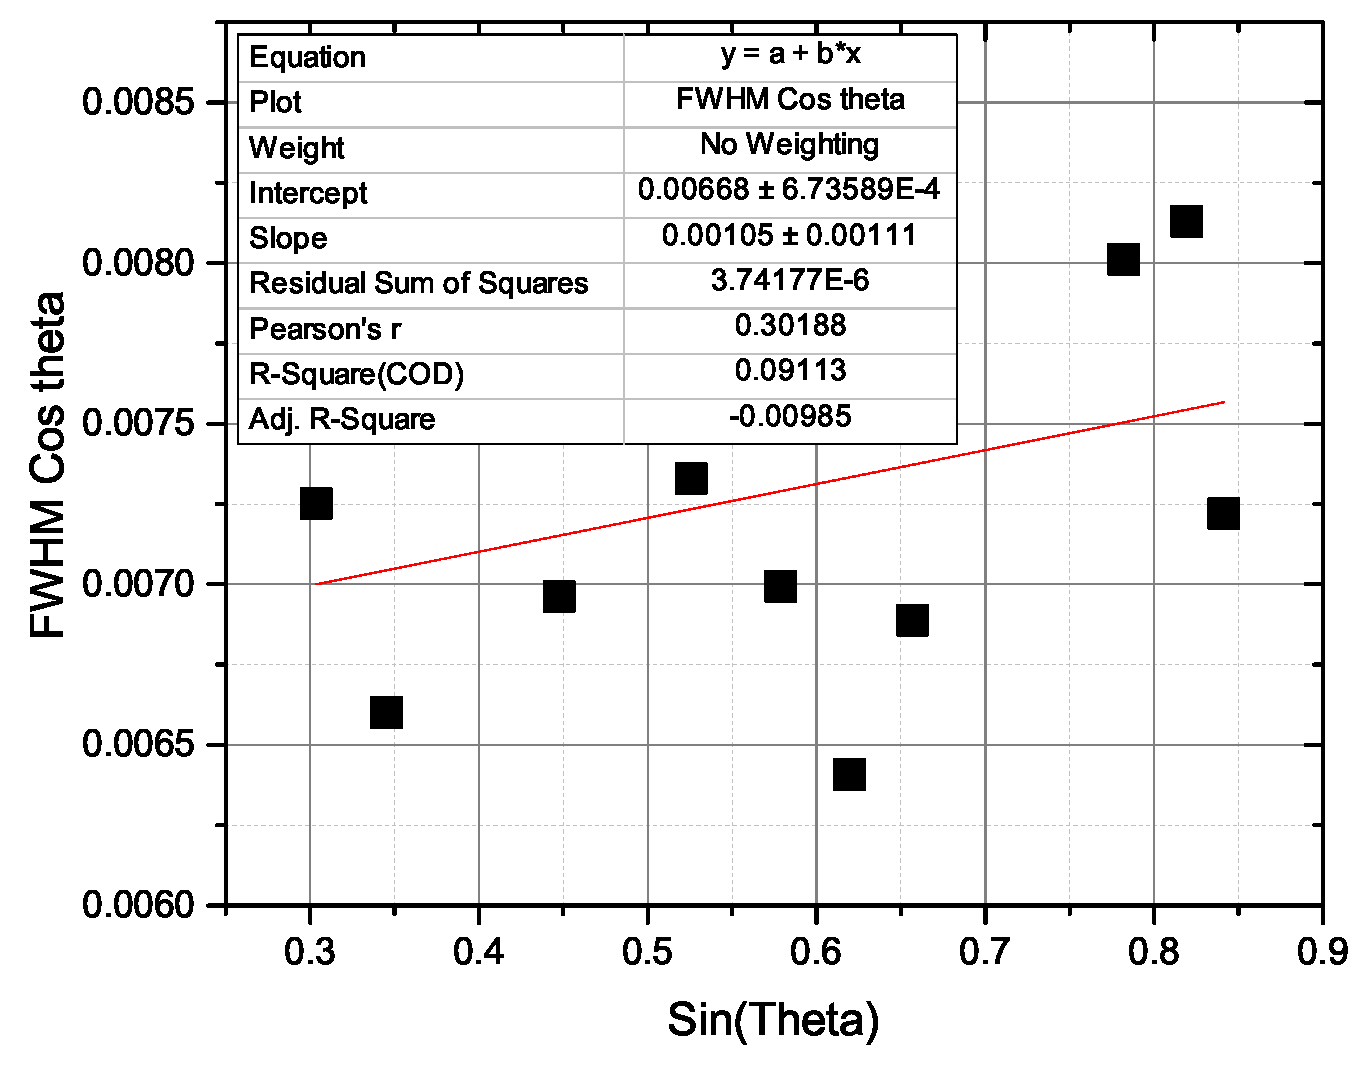
\includegraphics[width=0.50\textwidth]{/XRD/Images/WH-Ti-6242}
        \caption{Ti-6242 As Received; Surface}
    \label{fig:EDM-Cut}
\end{figure}

% Introduction
\documentclass[../main.tex]{subfiles}
\begin{document}


\chapter{Introduction}
% Literature Review
\chapter{Literature Review}
Titanium can exist in two allotropic forms: alpha (a hexagonal close-packed crystal structure) and beta (a body-cen- tered cubic structure) (Ref 7.1–7.4). In pure tita- nium, the alpha (a) phase is stable up to 880 °C (1620 °F), at which point it transforms to the beta (b) phase; the beta phase is stable from 880 °C (1620 °F) to the melting point. At room temperature, pure titanium consists of the alpha phase. However, the alloys can contain alpha, mixtures of alpha and beta, or beta phases, de- pending on the alloy content and conditions. Thus, the alloys are classified into these structural types: alpha ($\alpha$), alpha-beta ($\alpha$-$\beta$), and beta ($\beta$).


There are two major breakdowns in classifying the alloying elements. These are based on: A- whether or not the alloying elements are between the titanium atoms (interstitial) or replace titanium atoms (substitutional), and B-whether the alpha phase is entered preferentially (alpha stabilizing) or the beta phase is entered preferentially (beta stabilizing). The beta stabilizing elements generally are classified further, depending on whether or not there is a continuous series of solid solution between the alloying element and beta titanium (beta iso- morphous), or the beta phase decomposes eutectoidally (beta eutectoid).
% Experimental Details
\chapter{Experimental Details}
\section{Titanium 6246 Alloy} 

\begin{figure}[H]
    \centering
    \begin{subfigure}{0.40\textwidth}
        \includegraphics[width=\textwidth]{\Photos{"Ti6246 [uncut]"}}
        \caption{Ti-6246 As Received; Surface}
        \label{fig:2a}
    \end{subfigure}
    ~
    \begin{subfigure}{0.40\textwidth}
        \includegraphics[width=\textwidth]{\Photos{{"Ti6246 [uncut-cs]"}}
        \caption{Ti-6246 As Received; Cross-Section}
        \label{fig:2b}
    \end{subfigure}
    %\caption{}
    \label{fig:As-Received}
\end{figure}

\section{Titanium 6242 Alloy} 

\begin{figure}[H]
    \centering
        \includegraphics[width=0.50\textwidth]{\Photos{"Ti6242-1-Flat"}}
        \caption{Ti-6242 As Received; Surface}
    \label{fig:EDM-Cut}
\end{figure}


\subsection{EDM Cutting}
The samples were cut in EDM. To identify Surface and Cross-Section samples, an additional L-shaped groove was made on all the Cross-Section samples. 

\begin{figure}[H]
    \centering
        \includegraphics[width=\textwidth]{\Photos{"Ti6246 [cut-EDM]"}}
        \caption{Ti-6246 EDM Cut; Different Profile for surface and Cross-Section}
    \label{fig:EDM-Cut}
\end{figure}

The samples were cut in EDM. To identify Surface and Cross-Section samples, an additional groove was made on all the Cross-Section samples. 
\\
The Surface and the Cross-Section microstructure are taken from the same sample. The Cross-Section has a thin line to differentiate it from the Surface.


\begin{figure}[H]
    \centering
    \begin{subfigure}{0.40\textwidth}
        \includegraphics[width=\textwidth]{\Photos{"Ti6242-1-EDM Cut-1.1.1-Top"}}
        \caption{Ti-6242 EDM Cut; Surface}
        \label{fig:2a}
    \end{subfigure}
    ~
    \begin{subfigure}{0.40\textwidth}
        \includegraphics[width=\textwidth]{\Photos{"Ti6242-1-EDM Cut-1.1.1-CS"}}
        \caption{Ti-6242 EDM Cut; Cross-Section}
        \label{fig:2b}
    \end{subfigure}
    %\caption{}
    \label{fig:Ti-6242 EDM Cut; Cross-Section}
\end{figure}

\subsection{Slow Speed Cutting of Cross-Section Sample}

\begin{figure}[H]
    \centering
        \includegraphics[width=\textwidth]{\Photos{"Slow Speed Cutting"}}
        \caption{Ti-6246 Slow Speed Cutting}
    \label{fig:slow-speed-Cut}
\end{figure}



\section{Initial Microstructure}
Polishing - 600, 800, 1000, 1200, 1500, 2000 grit size. \\
Etchant - Equal parts of Methanol + HF + HCl + HNO$_{3}$ \\
Etching Time - 5 seconds

\subsection{Ti-6246}

\begin{figure}[H]
    \centering
    \begin{subfigure}{0.49\textwidth}
        \includegraphics[width=\textwidth]{\HeatTreatment{"Ti6246-1.1-Top (500x)"}}
        \caption{Ti-6246 Surface; Area Fraction - 33.87\%}
        \label{fig:a-As-Received-micro}
    \end{subfigure}
    ~
    \begin{subfigure}{0.49\textwidth}
        \includegraphics[width=\textwidth]{\HeatTreatment{"Ti6246-1.1.1-CS (500x)"}}
        \caption{Ti-6246 Cross-Section; Area Fraction - 56.79\%}
        \label{fig:b-As-Received-micro}
    \end{subfigure}
  
    \caption{Microstructure of Ti-6246 Alloy; Magnification - 500x}
    \label{fig:As-Received-micro}
\end{figure}

\subsection{Ti-6242}

\begin{figure}[H]
    \centering
    \begin{subfigure}{0.49\textwidth}
        \includegraphics[width=\textwidth]{\HeatTreatment{"Ti6242-1.2-Top-5(500x)"}}
        \caption{Ti-6242 Surface}
        \label{fig:Ti-6242 Surface}
    \end{subfigure}
    ~
    \begin{subfigure}{0.49\textwidth}
        \includegraphics[width=\textwidth]{\HeatTreatment{"Ti6242-1.1-CS-5(500x)"}}
        \caption{Ti-6242 Cross-Section}
        \label{fig:Ti-6242 Cross-Section}
    \end{subfigure}
  
    \caption{Microstructure of Ti-6242 Alloy; Magnification - 500x}
    \label{fig:As-Received}
\end{figure}

\iffalse
\begin{figure}[H]
    \centering
    \begin{subfigure}{0.49\textwidth}
        \includegraphics[width=\textwidth]{\HeatTreatment{"Ti6246-1.1-Top (1000x)"}}
        \caption{Ti-6246 Surface}
        \label{fig:2a}
    \end{subfigure}
    ~
    \begin{subfigure}{0.49\textwidth}
        \includegraphics[width=\textwidth]{\HeatTreatment{"Ti6246-1.1.1-CS (1000x)"}}
        \caption{Ti-6246 Cross-Section}
        \label{fig:2a}
    \end{subfigure}
  
    \caption{SEM Microstructure of Ti-6246 Alloy; Magnification - 1000x}
    \label{fig:As-Received-SEM}
\end{figure}

\fi

\section{Area Fraction Analysis}
Area fraction is given by:
\begin{equation}
V_{v} = \dfrac{\sum A_{A}}{A_{T}}
\end{equation} 

Error is given by:
\begin{equation}
E_{A}^{2} = \dfrac{1}{N}\left[ 1+ \left( \dfrac{\sigma}{\overline A} \right)^{2} \right]
\end{equation} 

\subsection{ImageJ}

\subsubsection{Ti-6246}
\begin{figure}[H]
    \centering
    \begin{subfigure}{0.49\textwidth}
        \includegraphics[width=\textwidth]{\HeatTreatment{"Ti6246-1.1.1-CS (500x) - Threshold"}}
        \caption{Ti-6246 Threshold}
        \label{fig:Ti-6246 Threshold}
    \end{subfigure}
    ~
    \begin{subfigure}{0.49\textwidth}
        \includegraphics[width=\textwidth]{\HeatTreatment{"Ti6246-1.1.1-CS (500x) - Outline"}}
        \caption{Ti-6246 Outline}
        \label{fig:Ti-6246 Outline}
    \end{subfigure}
  
    \caption{Microstructure of Ti-6246 Alloy; Magnification - 500x}
    \label{fig:As-Received-SEM}
\end{figure}

% Area fraction of $\alpha$-phase was measured to be 34.7\% and 
Area fraction of equiaxed $\alpha$-phase was measured to be 23.6\%.
\\
Mean Area - 22.58 $\mu m^{2}$, Standard Deviation - 34.81 $\mu m^{2}$, E$_{A}$ - 0.285 (95\% Accuracy - ie., 2E$_{A}$). 

\subsubsection{Ti-6242}
\begin{figure}[H]
    \centering
    \begin{subfigure}{0.49\textwidth}
        \includegraphics[width=\textwidth]{\HeatTreatment{"Ti6242-1.1-CS-5(500x) - Threshold"}}
        \caption{Ti-6242 Threshold}
        \label{fig:Ti-6242 Threshold}
    \end{subfigure}
    ~
    \begin{subfigure}{0.49\textwidth}
        \includegraphics[width=\textwidth]{\HeatTreatment{"Ti6242-1.1-CS-5(500x) - Outline"}}
        \caption{Ti-6242 Outline}
        \label{fig:Ti-6242 Outline}
    \end{subfigure}
  
    \caption{Microstructure of Ti-6242 Alloy; Magnification - 500x}
    \label{fig:As-Received}
\end{figure}


%The area fraction of $\alpha$-phase is 67.4\%. \\
The area fraction of equiaxed $\alpha$-phase is 27.9\% \\
Mean Area - 397.17 $\mu m^{2}$, Standard Deviation - 275.56 $\mu m^{2}$, E$_{A}$ - 0.703 (95\% Accuracy - ie., 2E$_{A}$).

\subsection{Matlab}

\subsubsection{Ti-6246}

\begin{figure}[H]
    \centering
    \begin{subfigure}{0.49\textwidth}
        \includegraphics[width=\textwidth]{\HeatTreatment{"Ti6246-1.1.1-CS (500x)-MatLab"}}
        \caption{Ti-6246 MatLab}
        \label{fig:Ti-6246 Threshold}
    \end{subfigure}
    ~
    \begin{subfigure}{0.49\textwidth}
        \includegraphics[width=\textwidth]{\HeatTreatment{"Ti6246-1.1.1-CS (500x)-MatLab-Threshold"}}
        \caption{Ti-6246 MatLab Threshold}
        \label{fig:Ti-6246 Outline}
    \end{subfigure}
  
    \caption{Microstructure of Ti-6246 Alloy; Magnification - 500x}
    \label{fig:As-Received-SEM}
\end{figure}

% Area fraction of $\alpha$-phase was measured to be 34.7\% and 
Area fraction of equiaxed $\alpha$-phase was measured to be 19.8\%.
\\
Mean Area - 22.58 $\mu m^{2}$, Standard Deviation - 34.81 $\mu m^{2}$, E$_{A}$ - 0.285 (95\% Accuracy - ie., 2E$_{A}$). 


\section{Tensile Test}

\begin{table}[H]
\centering
\resizebox{\textwidth}{!}{%
\begin{tabular}{ccccccc}
\hline
\textbf{Sample ID} & \textbf{Diameter (mm)} & \textbf{Gauge Length (mm)} & \textbf{Strain Rate (s$ ^{-1} $)} & \textbf{Cross-head Speed (mm/s)} & \textbf{Yield Strength (MPa)} \\ \hline
\hypertarget{Ti6242-1.2-TS}{Ti6242-1.2-TS} & - & - & - & - & & \\ \hline
Ti6242-1.3-TS & - & - & - & - & & \\ \hline
Ti6242-1.4-TS & 4.043 & 20 & 0.0333 & 0.666 & 956.53 @0.2\% \\ \hline
Ti6242-1.5-TS & 4.037 & 20 & 0.0333 & 0.666 & 961.63 @0.2\% \\ \hline
\end{tabular}%
}
\caption{Tensile Test of Ti-6242 Alloy}
\label{table:Tensile-Test-Ti-6242}
\end{table}

Example table row hyperlinking - \hyperlink{Ti6242-1.2-TS}{Test}. %https://tex.stackexchange.com/a/356939

\begin{table}[H]
\centering
\resizebox{\textwidth}{!}{%
\begin{tabular}{c|c|c|}
\cline{2-3}
 & \textbf{My Work} & \textbf{Arunima's Work} \\ \hline
\multicolumn{1}{|c|}{\textbf{Test Type}} & Tensile Test & Compression Test \\ \hline
\multicolumn{1}{|c|}{\textbf{Dimensions}} & \multicolumn{1}{l|}{4 mm (Diameter), 20 mm (Gauge Length)} & \multicolumn{1}{l|}{6 mm x 6 mm x 11 mm (Aspect Ratio - 1.83)} \\ \hline
\multicolumn{1}{|c|}{\textbf{Yield Strength (MPa)}} & 960 (@0.2\%) & 902 (@0.2\%, Thesis), 1045 (@5\%, Presentation) \\ \hline
\multicolumn{1}{|c|}{\textbf{Strain Rate (s$ ^{-1} $)}} & 3.3 x 10$^{-2}$ & 10$^{-3}$ \\ \hline
\end{tabular}%
}
\caption{Yield Strength Comparison with Arunima's Work}
\label{table:Yield Strength Comparison with Arunima's Work}
\end{table}

\begin{figure}[H]
    \centering
    \begin{subfigure}{0.40\textwidth}
        \includegraphics[width=\textwidth]{\TensileTest{Ti6242-1.4-TS-Graph}}
        \caption{Ti6242-1.4 As Received Tensile Test}
        \label{fig:2a}
    \end{subfigure}
    ~
    \begin{subfigure}{0.40\textwidth}
        \includegraphics[width=\textwidth]{\TensileTest{Ti6242-1.5-TS-Graph}}
        \caption{Ti6242-1.5 As Received Tensile Test}
        \label{fig:2b}
    \end{subfigure}
    \\
    \begin{subfigure}{0.40\textwidth}
        \includegraphics[width=\textwidth]{\TensileTest{Tensile Test [Arunima Banerjee]}}
        \caption{Ti6242 As received Tensile Test by Arunima} 
        \label{fig:2b}
    \end{subfigure} 
     
    \caption{Tensile Test of as received Ti-6242 @0.0333 s$ ^{-1} $}
    \label{fig:Tensile-Test-6242}
\end{figure}

%%%%%%%%%%%%%%%%%%%%%%%%%%%% Fatigue Test %%%%%%%%%%%%%%%%%%%%%%%%%%%%%%
\section{Fatigue Test}
\label{sec:Fatigue Test}

\subsection{Ti-6242}
\label{subsec:Fatigue Test -  Ti-6242}

\subsubsection{S-N Curve}
\label{subsec:Fatigue Test -  Ti-6242 - S-N Curve}


\begin{figure}[H]
    \centering
        \includegraphics[width=0.50\textwidth]{\FatigueTest{S-N curve}}
        \caption{S-N Curve (Ti-6242 Fatigue Test)}
    \label{fig:fatigue-test-sn-curve}
\end{figure}

%%%%%%%%%%%%%%%%%%%%%%%%%%%% Heat Treatment %%%%%%%%%%%%%%%%%%%%%%%%%%%%%%
\section{Heat Treatment}
\label{sec:Heat Treatment}

\subsubsection{Ti-6242}
\begin{figure}[H]
    \centering
    \begin{subfigure}{0.49\textwidth}
        \includegraphics[width=\textwidth]{\HeatTreatment{"Ti6242-1.1-CS-5(500x)-MatLab"}}
        \caption{Ti-6242 Threshold}
        \label{fig:Ti-6242 Threshold}
    \end{subfigure}
    ~
    \begin{subfigure}{0.49\textwidth}
        \includegraphics[width=\textwidth]{\HeatTreatment{"Ti6242-1.1-CS-5(500x)-MatLab-Threshold"}}
        \caption{Ti-6242 Threshold MatLab}
        \label{fig:Ti-6242 Threshold MatLab}
    \end{subfigure}
  
    \caption{Microstructure of Ti-6242 Alloy; Magnification - 500x}
    \label{fig:As-Received}
\end{figure}


The area fraction of equiaxed $\alpha$-phase is 33.34\% \\
Mean Area - 397.17 $\mu m^{2}$, Standard Deviation - 275.56 $\mu m^{2}$, E$_{A}$ - 0.703 (95\% Accuracy - ie., 2E$_{A}$).
\\
\textbf{Note:} The area fraction of Ti6242 measured at 100x magnification gave the lowest error and 500x magnification gave the highest error. So all measurements were made at 100x.

% Results and Discussion
\chapter{Results and Discussion}
% Summary And Conclusions
\chapter{Summary and Conclusions}











\chapter{Scope for Future Work}

\fi
%%%%%%%%%%%%%%%%%%%%%%%%%%%%%%%%%%%%%%%%%%%%%%%%%%%%%%%%%%%%%%%%%%%%%%
%							 Appendix
%%%%%%%%%%%%%%%%%%%%%%%%%%%%%%%%%%%%%%%%%%%%%%%%%%%%%%%%%%%%%%%%%%%%%%
\appendix
%\chapter{My Appendix}
%%%%%%%%%%%%%%%%%%%%%%%%%%%%%%%%%%%%%%%%%%%%%%%%%%%%%%%%%%%%%%%%%%%%%%
% 						Bibliography or References
%%%%%%%%%%%%%%%%%%%%%%%%%%%%%%%%%%%%%%%%%%%%%%%%%%%%%%%%%%%%%%%%%%%%%%
%\bibliographystyle{plainnat}

\bibliography{references}

\end{document}